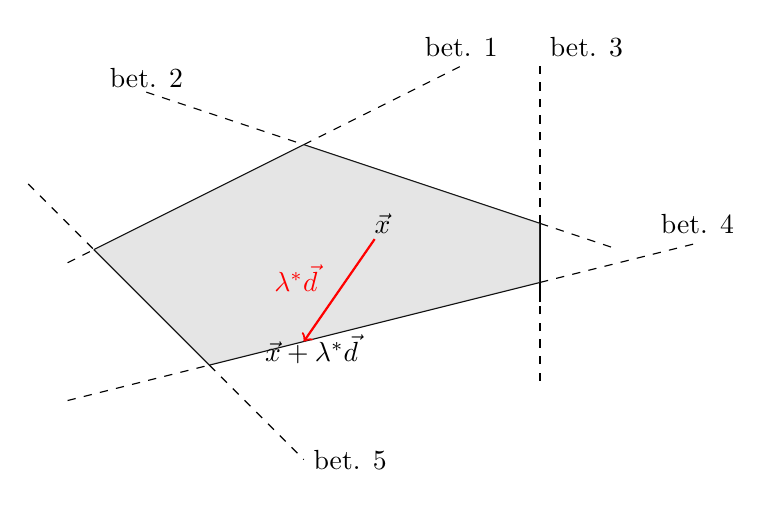
\begin{tikzpicture}[ latex
  s/.style={width=0}]

  %ligning 1
	\draw[domain=-1:-2/3,variable=\x,dashed] 	plot({\x},{0.5*\x+1});
	\draw[domain=-2/3:2,variable=\x] 			plot({\x},{0.5*\x+1});
	\draw[domain=2:4,variable=\x,dashed] 	plot({\x},{0.5*\x+1}) node[above] {bet. 1};
	
  %ligning 2
  	\draw[domain=0:2,variable=\x,dashed] 	plot({\x},{-(1/3)*\x+8/3}) node[above] at (0,2.6) {bet. 2} ;
	\draw[domain=2:5,variable=\x] 			plot({\x},{-(1/3)*\x+8/3});
	\draw[domain=5:6,variable=\x,dashed] 	plot({\x},{-(1/3)*\x+8/3});
	

  %ligning 3
  	\draw[domain=-1:0,variable=\y,dashed] 	plot({5},{\y});
	\draw[domain=0:1,variable=\y] 			plot({5},{\y});
	\draw[domain=1:3,variable=\y,dashed] 	plot({5},{\y}) node[above right] {bet. 3};
	
  %ligning 4
	\draw[domain=-1:4/5,variable=\x,dashed] 	plot({\x},{0.25*\x-1});
	\draw[domain=4/5:5,variable=\x] 			plot({\x},{0.25*\x-1});
	\draw[domain=5:7,variable=\x,dashed] 	plot({\x},{0.25*\x-1}) node[above] {bet. 4};
	
  %ligning 5
  	\draw[domain=-1.5:-2/3,variable=\x,dashed] 	plot({\x},{-\x}) ;
	\draw[domain=-2/3:4/5,variable=\x] 			plot({\x},{-\x});
	\draw[domain=4/5:2,variable=\x,dashed] 	plot({\x},{-\x}) node[right] {bet. 5} ;

  %løsningsmængden skraveret
	\fill[gray!80,nearly transparent] (4/5,-4/5) -- (-2/3,2/3) -- (2,2) -- (5,1) --(5,0.25) --  cycle;
	
  % vektor x
	\node[] (x) at (3,1) {$\vec{x}$};
	\draw[thick, color=red, ->](2.9,0.8) -- (2,-0.5) node[above, yshift=0.5 cm, xshift=-0.1 cm] {$\lambda^* \vec{d}$} ;
	\node[] (x) at (2.1, -0.6) {$\vec{x}+\lambda^* \vec{d}$};
 
\end{tikzpicture}